\chapter[Topic: Annuities / cash flows with non-contingent payments]{Topic: Annuities / cash flows with non-contingent payments (exam weight)}

\subsection{Information}

\begin{distributions}[Objective]
The Candidate will be able to calculate present value, current value, and accumulated value for sequences of non-contingent payments.
\end{distributions}

\begin{outcomes}[Learning outcomes]
The candidate will be able to:
\begin{enumerate}[label = \alph*)]
	\item	Define and recognize the \textit{definitions} of the following terms:
		\begin{multicols*}{2}
		\begin{itemize}[leftmargin = *]
		\item	Annuity-immediate;
		\item	Annuity-due;
		\item	Perpetuity;
		\item	Payable $m$-thly or continously;
		\item	Level payment annuity;
		\item	Arithmetic increasing/decreasing annuity;
		\item	Geometric increasing/decreasing annuity;
		\item	Term of annuity;
		\end{itemize}
		\end{multicols*}
	\item	For each of the following types of annuity / cash flows, given sufficient information of :
		\begin{multicols*}{2}
		\begin{itemize}[leftmargin = *]
		\item	Immediate or due;
		\item	Present value;
		\item	Futur value;
		\item	Current value;
		\item	Interest rate;
		\item	Payment amount;
		\item	Term of annuity,
		\end{itemize}
		\end{multicols*}
		calculate any remaining item. 
	\item[]	The types are:
		\begin{itemize}[leftmargin = *]
		\item	Level annuity, finite term;
		\item	Level perpetuity;
		\item	Non-level annuities / cash flows;
			\begin{itemize}
			\item	Arithmetic progression, finite term and perpetuity;
			\item	Geometric progression, finite term and perpetuity;
			\item	Other non-level annuities / cash flows.
			\end{itemize}
		\end{itemize}
\end{enumerate}
\end{outcomes}

\begin{ASM_chapter}[Related lessons ASM]
Section 3: Annuities
\begin{itemize}
	\item	\nameref{L.-3a}
	\item	\nameref{L.-3b}
	\item	\nameref{L.-3c}
	\item	\nameref{L.-3d}
	\item	\nameref{L.-3e}
	\item	\nameref{L.-3f}
	\item	\nameref{L.-3g}
	\item	\nameref{L.-3h}
	\item	\nameref{L.-3i}
\end{itemize}
Section 4: Complex Annuities
\begin{itemize}
	\item	\nameref{L.-4a}
	\item	\nameref{L.-4b}
	\item	\nameref{L.-4c}
	\item	\nameref{L.-4d}
	\item	\nameref{L.-4e}
	\item	\nameref{L.-4f}
	\item	\nameref{L.-4g}
	\item	\nameref{L.-4h}
	\item	\nameref{L.-4i}
	\item	\nameref{L.-4j}
	\item	\nameref{L.-4k}
	\item	\nameref{L.-4l}
	\item	\nameref{L.-4m}
\end{itemize}
\end{ASM_chapter}
%
%\begin{YTB_vids}[Vidéos YouTube]
%\begin{itemize}
%	\item	
%\end{itemize}
%\end{YTB_vids}

\subsection{Résumés des chapitres}

\begin{CHPT_SUMM_AUTO}[label = {L.-3a}]{3a. The Geometric Series Trap}
Remember the formula for geometric series in words:
\begin{align*}
	r^{10} + r^{20} + \dots + r^{10n}
	&=	r^{10}\frac{1 - r^{n}}{1 - r}	\\
	&=	(\text{first term}) \frac{1 - (\text{ratio})^{\text{nb. of terms}}}{1 - (\text{ratio})}
\end{align*}
	\begin{itemize}
		\item	
	\end{itemize}
\end{CHPT_SUMM_AUTO}

\begin{CHPT_SUMM_AUTO}[label = {L.-3b}]{3b. Annuity-Immediate and Annuity-Due}
	\begin{itemize}
		\item	Origin of the word: annu(us) latin for \og yearly \fg{};
		\item	Standard annuity formulas for $\ax{\angln}, \ax**{\angln}, \sx{\angln}, \sx**{\angln}$;
		\item	Interesting to note the relations between them however.
	\end{itemize}
\setlength{\mathindent}{-1cm}

\textbf{Formulas}
	\begin{minipage}[ht]{0.4\linewidth}
	\begin{align*}
	\ax**{\angln}	
	&=	1 + v + v^{2} + \dots + v^{n - 1}	\\
	&=	\frac{1 - v^{n}}{1 - v}	\\
	&=	\frac{1 - v^{n}}{d}	\\
	\ax{\angln}	
	&=	v + v^{2} + \dots + v^{n - 1} + v^{n}	\\
	&=	v\left(\frac{1 - v^{n}}{1 - v}\right)	\\
	&=	\frac{1 - v^{n}}{i}	
	\end{align*}	
	\end{minipage}
	\begin{minipage}[ht]{0.6\linewidth}
		\begin{align*}
	\sx**{\angln}	
	&=	(1 + i) + \dots + (1 + i)^{n - 1} + (1 + i)^{n}	\\	
	&=	(1 + i)\left(\frac{1 - (1 + i)^{n}}{1 - (1 + i)}\right)	\\
	&=	\frac{(1 + i)^{n} - 1}{d}	\\
	\sx{\angln}	
	&=	1 + (1 + i) + \dots + (1 + i)^{n - 1}	\\
	&=	\frac{1 - (1 + i)^{n}}{1 - (1 + i)}	\\
	&=	\frac{(1 + i)^{n} - 1}{i}	
	\end{align*}
	\end{minipage}

\textbf{Relations}
	\begin{minipage}[ht]{0.5\linewidth}
	\begin{align*}
	\ax**{\angln}	
	&=	(1 + i) \ax{\angln}	\\
	&=	\ax{\angl{n - 1}} - 1
	\end{align*}	
	\end{minipage}
	\begin{minipage}[ht]{0.5\linewidth}
		\begin{align*}
	\sx**{\angln}	
	&=	(1 + i) \sx{\angln}	\\
	&=	\sx{\angl{n + 1}} - 1	
	\end{align*}
	\end{minipage}
	\setlength{\mathindent}{1cm}
\end{CHPT_SUMM_AUTO}

\begin{CHPT_SUMM_AUTO}[label = {L.-3c}]{3c. The Great Confusion: Annuity-Immediate and Annuity-Due}

\begin{itemize}[leftmargin = *]
		\item	Defining whether annuities are due or immediate based on \textit{when payments are made} is deceptive, it is more precise to define it based on the \textit{valuation date}.
\end{itemize}

\begin{FORMULA_SUMM}{Annuity}
An annuity is called an \textbf{annuity-immediate} if, in determining its present value, the valuation date is \textbf{\textit{one period before}} the first payment (symbol $\ax{\angln}$). An annuity is called an \textbf{annuity-due} if, in determining its present value, the valuation date is \textit{\textbf{on}} the date of the first payment (symbol $\ax*{\angln}$).

\tcbline

An annuity is called an \textbf{annuity-immediate} if, in determining its accumulated value, the valuation date is \textit{\textbf{on}} the date of the last payment (symbol $\sx{\angln}$). An annuity is called an \textbf{annuity-due} if, in determining its accumulated value, the valuation date is \textit{\textbf{one period after}} the date of the last payment (symbol $\sx*{\angln}$).
\end{FORMULA_SUMM}

\begin{itemize}[leftmargin = *]
		\item	Important to distinguish dates in time from the number of payments.
		\item[]	For example, if we're the 1st of January in 2000 and annual payments are made on the 1st of January from 2006 to 2010 then the AV on the date of the last deposit is $\sx{\angl{5}}$ and not $\sx{\angl{10}} - \sx{\angl{5}}$ nor $\sx{\angl{2010}}$, etc.
		\item	Better to set up equations of value with annuity-immediate than annuity-due.
\end{itemize}
\end{CHPT_SUMM_AUTO}

\begin{CHPT_SUMM_AUTO}[label = {L.-3d}]{3d. Deferred Annuities}
\begin{itemize}[leftmargin = *]
		\item	An $n$-year annuity deferred $r$ years $\ax[r|]{n} = v^{r} \ax{n}$.
		\item	Can interpret as "go to to time $r$ and start paying what the symbol to the right says".
		\item	Can also interpret by playing "Now you see it ..." and redefining $\ax[r|]{n} = \ax{n + r} - \ax{r}$:
		\begin{center}
			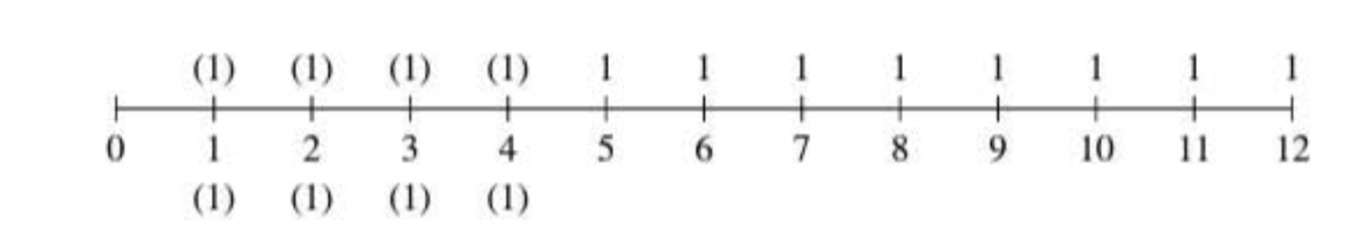
\includegraphics[scale=0.4]{img/deferred-annuities-nowyouseeit.png}
		\end{center}
		\item[]	The value is thus $\ax[4|]{8} = \ax{12} - \ax{4}$ in the example.		
\end{itemize}

\begin{FORMULA_SUMM}{Deferred Annuities}
\begin{align*}
	\ax[r|]{n} &\equiv \ax**[r + 1| ]{n}	\\
	v^{r} \ax{n}	&\equiv	v^{r + 1} \ax**{n}	\\
	\ax{n + r} - \ax{r}
\end{align*}
\end{FORMULA_SUMM}
\end{CHPT_SUMM_AUTO}

\begin{CHPT_SUMM_AUTO}[label = {L.-3e}]{3e. A Short-Cut Method for Annuities with "Block" Payments}
Block payments:
\begin{center}
	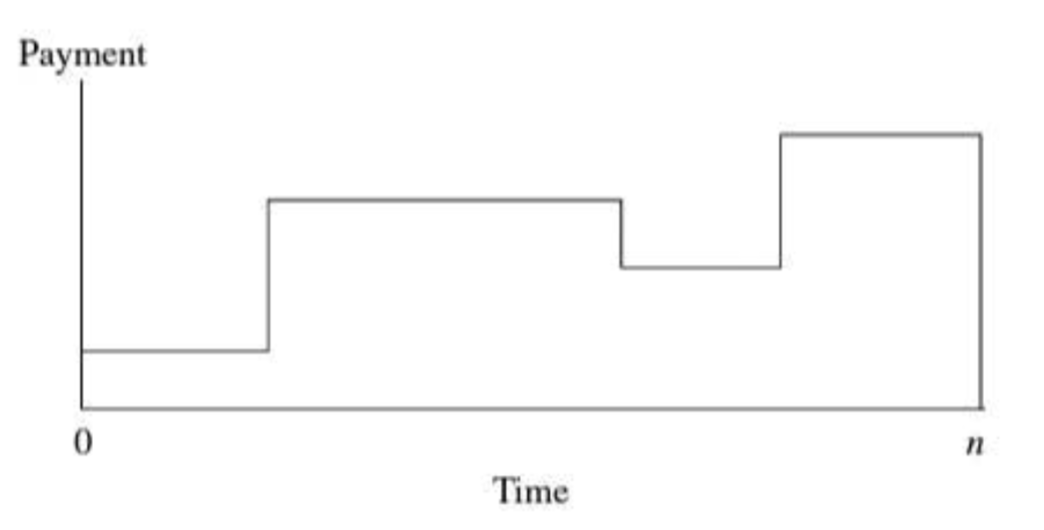
\includegraphics[scale=0.4]{img/deferred-annuities-blocks.png}
\end{center}

The long way is to calculate the payments by block and divide horizontally (first 8 payments, next 7 payments, etc.).
\begin{center}
	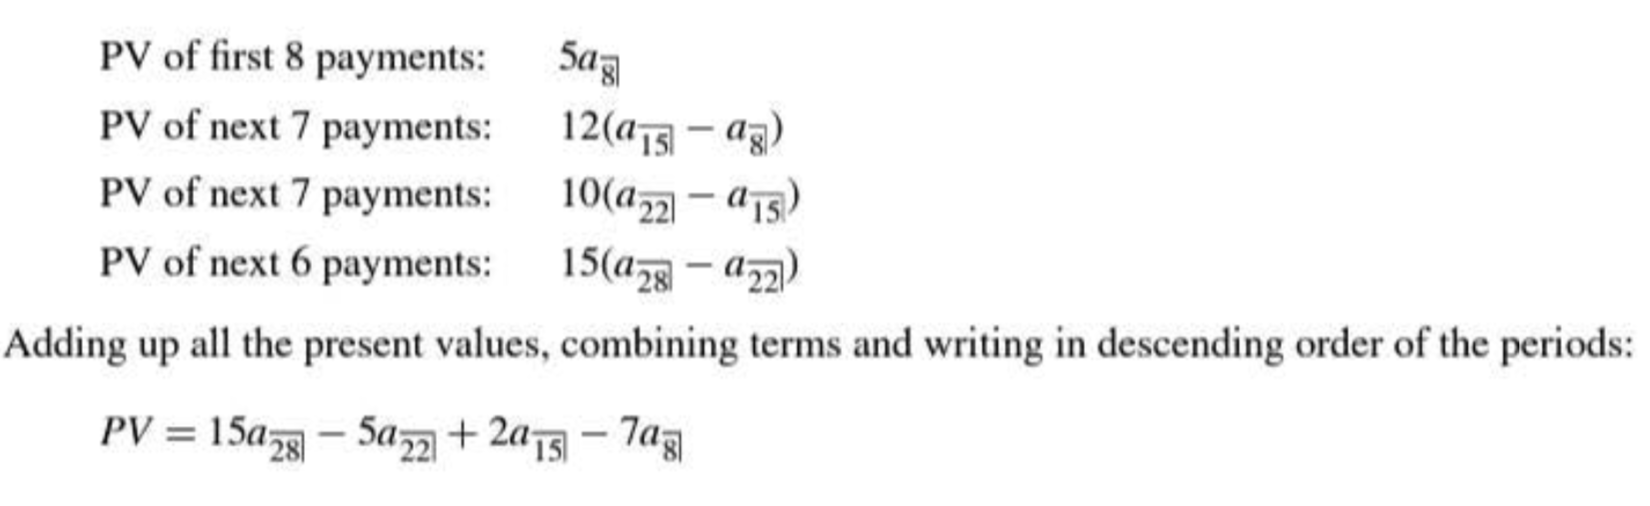
\includegraphics[scale=0.4]{img/deferred-annuities-blocks-long.png}
\end{center}
The short way starts from the end adding or decreasing annuities according to the change in payment amount.
\begin{center}
	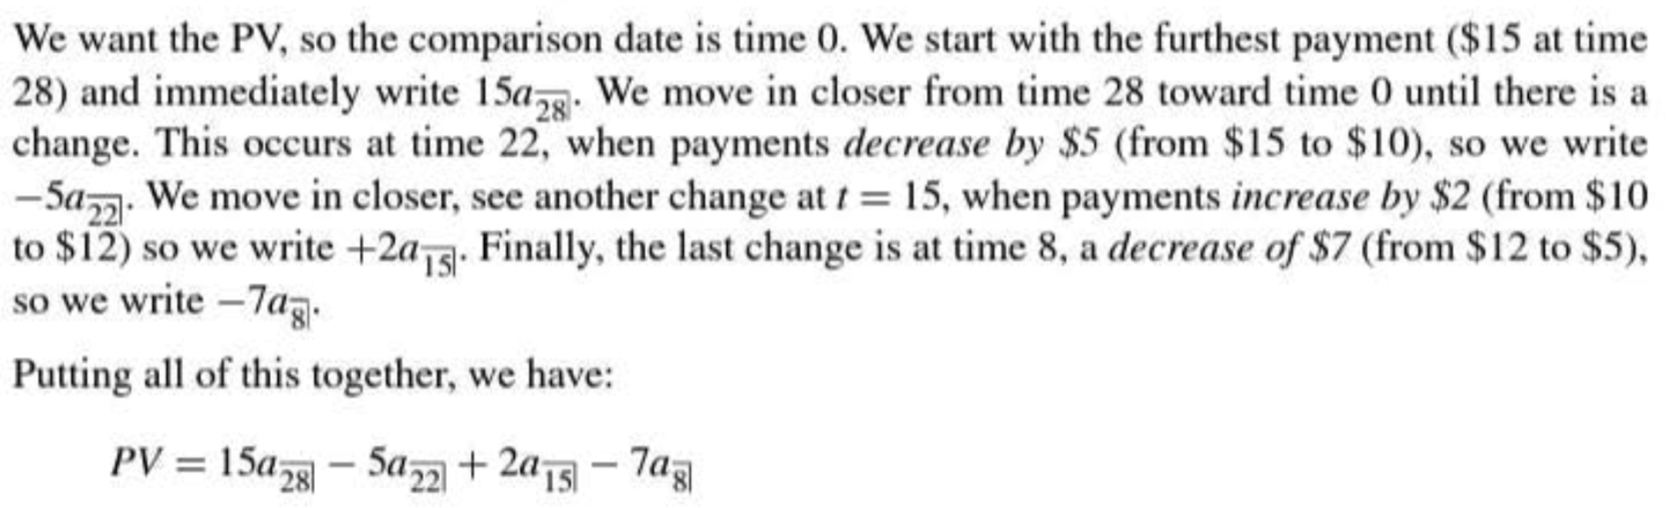
\includegraphics[scale=0.4]{img/deferred-annuities-blocks-short.png}
\end{center}

The same idea is maintained for the AV :
\begin{center}
	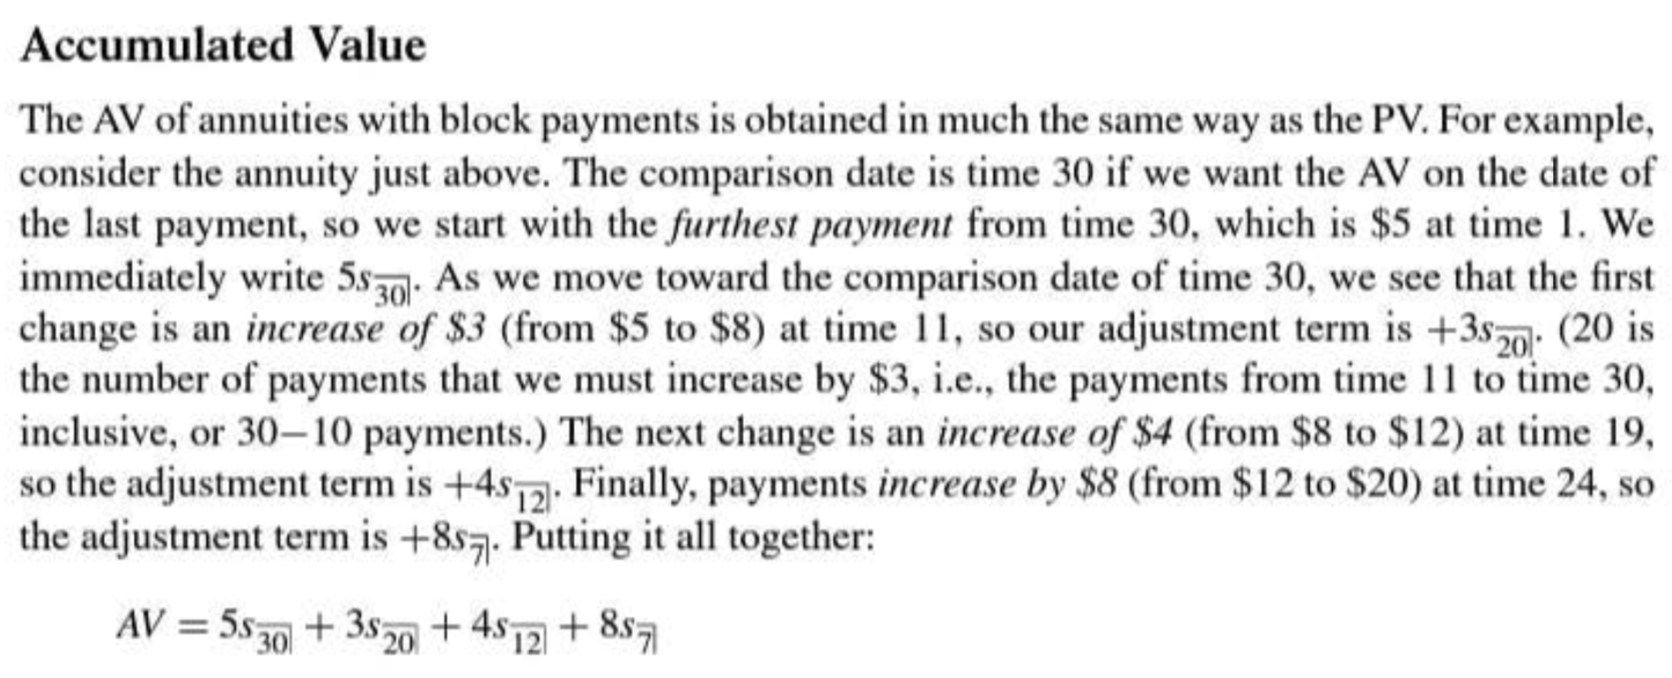
\includegraphics[scale=0.4]{img/deferred-annuities-blocks-AV.png}
\end{center}
\end{CHPT_SUMM_AUTO}

\begin{CHPT_SUMM_AUTO}[label = {L.-3f}]{3f. Perpetuities}
\begin{description}
	\item[Perpetuity-immediate]	$\ax{\angl{\infty}}	=	\frac{1}{i}$.
		One way to prove this is with the limit:
		\begin{align*}
		\underset{n \rightarrow \infty}{\lim} \ax{\angln}
		=	\underset{n \rightarrow \infty}{\lim} \left( \frac{1 - v^{n}}{i} \right)
		=	\frac{1}{i}
		\end{align*}
	\item[Perpetuity-due]	$\ax**{\angl{\infty}}	=	\frac{1}{d}$.
		One way to prove this is with the limit:
		\begin{align*}
		\underset{n \rightarrow \infty}{\lim} \ax**{\angln}
		=	\underset{n \rightarrow \infty}{\lim} \left( \frac{1 - v^{n}}{d} \right)
		=	\frac{1}{d}
		\end{align*}
	\item[link]		The PV of a perpetuity-due exceeds that of a perpetuity-immediate by the payment of 1 at time 0: 
		\begin{align*}
		\ax**{\angl{\infty}}	
		&=	1 + \ax{\angl{\infty}}	
		= 	1 + \frac{1}{i} 
		= 	\frac{1 + i}{i} 
		= 	\frac{1}{d}				\\
		\ax**{\angl{\infty}}	 - \ax{\angl{\infty}}	
		&=	\frac{1}{d} - \frac{1}{i} 
		=	1
		\end{align*}
	\item[Relationship]	
\end{description}
\end{CHPT_SUMM_AUTO}

\begin{CHPT_SUMM_AUTO}[label = {L.-3g}]{3g. The $\ax{\angl{2n}} / \ax{\angl{n}}$ Trick (and Variations)}
$\ax{\angl{2n}} / \ax{\angl{n}} = 1 + v^{n}$ and can proven several ways:\\

\textbf{Difference of squares}:
\begin{align*}
	\ax{\angl{2n}} / \ax{\angl{n}}
	&=	\frac{\frac{1 - v^{2n}}{i}}{\frac{1 - v^{n}}{i}}
	=	\frac{1 - v^{2n}}{1 - v^{n}}
	=	\frac{(1 - v^{n})(1 + v^{n})}{1 - v^{n}}
	=	1 + v^{n}
\end{align*}

\textbf{General reasoning}:
\begin{align*}
	\ax{\angl{2n}} / \ax{\angl{n}}
	&=	\frac{\ax{\angl{n}} + \ax[n|]{\angl{n}}}{\ax{\angl{n}}}
	&=	\frac{\ax{\angl{n}} + v^{n} \ax{\angl{n}}}{\ax{\angl{n}}}
	&=	\frac{\ax{\angl{n}}(1 + v^{n})}{\ax{\angl{n}}}
	&=	(1 + v^{n})
\end{align*}\\

This can be \textbf{generalized}:
\begin{align*}
	\ax{\angl{3n}} / \ax{\angl{n}}
	&=	\frac{\ax{\angl{n}} + \ax[n|]{\angl{n}} + \ax[2n|]{\angl{n}}}{\ax{\angl{n}}}
	=	\frac{\ax{\angl{n}} + v^{n} \ax{\angl{n}} + v^{2n} \ax{\angl{n}}}{\ax{\angl{n}}}	\\
	&=	\frac{\ax{\angl{n}}(1 + v^{n} + v^{2n})}{\ax{\angl{n}}}
	=	(1 + v^{n} + v^{2n})
\end{align*}
\end{CHPT_SUMM_AUTO}

\begin{CHPT_SUMM_AUTO}[label = {L.-3h}]{3h. What If the Rate Is Unknown?}
If the PV, number, and amount of payments of an annuity are known we can use the calculator tto solve for the interest rate.
\end{CHPT_SUMM_AUTO}

\begin{CHPT_SUMM_AUTO}[label = {L.-3i}]{3i. What If the Rate Varies?}
Be careful not to mix up the PV and AV interest accumulation.\\
Also, split up annuities if the interest rate varies so as not to make mistakes.
\end{CHPT_SUMM_AUTO}

\begin{CHPT_SUMM_AUTO}[label = {L.-4a}]{4a. Annuities with "Off-Payments" Part I}
\begin{description}
	\item[off-payments]	Payments which are less or more frequent than the interest period.\\
	For example:
		\begin{itemize}[leftmargin = *]
		\item	Payments of 1 at the end of each 5-year period over 40 years -> payments are \textit{less frequent} than the interest period of one year.
		\item	Payments of $\frac{1}{12}$ at the end of each month for 10 years -> payments are \textit{more frequent} than the interest period of one year.
		\end{itemize}
\end{description}

There are generally 2 approaches for handling these types of annuities
\begin{enumerate}
	\item	Use interest functions at the equivalent effective rate of interest for the \textbf{payment period}.
		\begin{itemize}[leftmargin = *]
		\item	Method is generally easier for numerical answers (i.e., most of the time).
		\end{itemize}
	\item	Use interest functions at the effective rate of interest \textbf{given in the problem}.
		\begin{itemize}[leftmargin = *]
		\item	Method is generally easier for symbolic answers.
		\end{itemize}
\end{enumerate}

The first method is this subsection. For example, monthly payments of $\frac{1}{12}$ paid at the end of each month for 10 years at an effective rate of 5\% per annum. 
\begin{itemize}[leftmargin = *]
	\item	First we find the equivalent rate:
				\begin{align*}
				1 + j	&= (1.05)^{1/12}	\\
					j	&=	0.4074\%
				\end{align*}
	\item	Then the PV:
				\begin{align*}
				PV	&=	\frac{1}{12} \ax{\angl{120}j}	\\
					&=	7.8971
				\end{align*}
\end{itemize}
\end{CHPT_SUMM_AUTO}

\begin{CHPT_SUMM_AUTO}[label = {L.-4b}]{4b. Annuities with "Off-Payments" Part II}
\begin{description}
	\item[Fission method]	When payments are less frequent than the interest period.
	\item[Fusion method]	When payments are more frequent than the interest period.
\end{description}

\tcbline
Example of Fission method:\\

Payments of 1 every 5 years for 40 years at an annual effective rate of 5\%.
What annual payment $R$ is equivalent to a payment of 1 every 5 years?
	\begin{align*}
	R \sx{\angl{5}}	&=	1	&
	&\Rightarrow	&
	R	&=	\frac{1}{\sx{\angl{5}}}
	\end{align*}

So the PV becomes:
	\begin{align*}
	\left(\frac{1}{\sx{\angl{5}}}\right)\ax{\angl{40}}
	\end{align*}
Thus we have done \og \textbf{fission} \fg{} by splitting up the payments into smaller payments.\\

It's very important to consider these 2 cases however:
	\begin{itemize}[leftmargin = *]
		\item	For payments which are in the beginning of the period, set up the equation as $P = R \ax**{\angln}$.
		\item	For payments which are in the end of the period, set up the equation as $P = R \sx{\angln}$.
	\end{itemize}
	
\tcbline

The fusion method leads to these formulas:
	\begin{align*}
	\ax{\angln}[(m)]
	&=	\frac{1 - v^{n}}{i^{(m)}}	
	=	\frac{i}{i^{(m)}}\ax{\angln}
	=	\sx{\angl{1}}[(m)]\ax{\angln}
	\end{align*}
	\begin{align*}
	\ax**{\angln}[(m)]
	&=	\frac{1 - v^{n}}{d^{(m)}}	
	=	\frac{i}{d^{(m)}}\ax{\angln}
	=	\sx**{\angl{1}}[(m)]\ax{\angln}
	\end{align*}
	\begin{align*}
	\sx{\angln}[(m)]
	&=	\frac{(1 + i)^{n} - 1}{i^{(m)}}	
	=	\frac{i}{i^{(m)}}\sx{\angln}
	=	\sx{\angl{1}}[(m)]\sx{\angln}
	\end{align*}
	\begin{align*}
	\sx**{\angln}[(m)]
	&=	\frac{(1 + i)^{n} - 1}{d^{(m)}}	
	=	\frac{i}{d^{(m)}}\sx{\angln}
	=	\sx**{\angl{1}}[(m)]\sx{\angln}
	\end{align*}
The reasoning is we accumulate the payment over the $m$ periods before treating it on an annual basis.

The same reasoning applies to perpetuities
	\begin{align*}
	\ax{\angl{\infty}}[(m)]		&=	\frac{1}{i^{(m)}}	&
	\ax**{\angl{\infty}}[(m)]	&=	\frac{1}{d^{(m)}}	&
	\ax{\angl{\infty}}[(m)] - \ax**{\angl{\infty}}[(m)]	&=	\frac{1}{m}	
	\end{align*}

\end{CHPT_SUMM_AUTO}

\begin{CHPT_SUMM_AUTO}[label = {L.-4c}]{4c. Avoiding the $m^{\text{thly}}$ Annuity Trap}
	\begin{itemize}[leftmargin = *]
		\item	It's important not to forget to have the payment be on the base as the annuity.
		\item	For example: payments of 100\$ paid at the end of every month over 10 years at an effective annual rate of 5\% means an annuity of $12 * 100 \ax{\angln}[(12)]$.
		\item[]	So the annuity is compounded 12 times a year with the "yearly" payment of 1200\$.
		\item	So the payment, or coefficient of the $\ax{\angln}$ term, is the \textbf{\textit{sum} of the payments} in \textbf{\textit{each} interest period}.
	\end{itemize}
\end{CHPT_SUMM_AUTO}

\begin{CHPT_SUMM_AUTO}[label = {L.-4d}]{4d. Continuous Annuities}
\begin{itemize}[leftmargin = *]
		\item	$\ax{\angln}[(m)]$ always requires a \textbf{total payment of 1} each year, regardless of the value of $m$.
		\item	The 1 is payable in $m$thly installments of $\frac{1}{m}$.
		\item	Thus we obtain this result as $m$ grows:
			\begin{align*}
			\underset{m \rightarrow \infty}{\lim} \ax{\angln}[(m)]
			&=	\underset{m \rightarrow \infty}{\lim} \left( \frac{1 - v^{n}}{i^{(m)}} \right)
			&=	\underset{m \rightarrow \infty}{\lim} \left( \frac{1 - v^{n}}{\delta} \right)
			&=	\ax*{\angln}
			\end{align*}
		\item	We also obtain the relation $\ax*{\angln} = \frac{i}{\delta}\ax{\angln}$.
\end{itemize}
\end{CHPT_SUMM_AUTO}

\begin{CHPT_SUMM_AUTO}[label = {L.-4e}]{4e."Double-Dots Cancel" (and so do "upper $m$'s")}
Given annuities being divided, we obtain:
	\begin{align*}
	\frac{\ax**{\angln}[(m)]}{\ax**{\angl{p}}[(m)]}
	&=	\frac{\ax**{\angln}}{\ax**{\angl{p}}}
	=	\frac{\ax{\angln}}{\ax{\angl{p}}}
	=	\frac{\ax{\angln}[(m)]}{\ax{\angl{p}}[(m)]}	
	=	\frac{1 - v^{n}}{1 - v^{p}}
	\end{align*}
\end{CHPT_SUMM_AUTO}

\begin{CHPT_SUMM_AUTO}[label = {L.-4f}]{4f. A Short Note on Remembering Annuity Formulas}
\begin{description}
	\item[PV]	all have $1 - v^{n}$ as the numerator.
	\item[FV]	all have $(1 + i)^{n} - 1$ as the numerator.
	\item[annuity \textit{\textbf{i}}mmediate]	has $i$ for \textbf{\textit{i}}mmediate $\frac{1 - v^{n}}{i}$.
	\item[annuity \textit{\textbf{d}}ue]	has $d$ for \textbf{\textit{d}}ue  $\frac{1 - v^{n}}{d}$.
	\item[compounded $m$ times a year]	changes $i$ for $i^{(m)}$ or $d$ for $d^{(m)}$.
	\item[compounded continuously]	changes $i$ and $d$ for $\delta$.
\end{description}
\end{CHPT_SUMM_AUTO}

\begin{CHPT_SUMM_AUTO}[label = {L.-4g}]{4g. The $\sx{\angln}$ Trap When Interest Variess}
\begin{itemize}[leftmargin = *]
	\item	If the force of interest is variable important not to fall into the trap of accumulating from 0.
	\item	$a(t)$ is the accumulation from 0 so the AV at time 5 of a payment at time 4 is $\frac{a(5)}{a(4)}$ and not $a(1)$.
\end{itemize}
\end{CHPT_SUMM_AUTO}

\begin{CHPT_SUMM_AUTO}[label = {L.-4h}]{4h. Payments in Arithmetic Progression}
\begin{description}
	\item[$P$]	First payment.
	\item[$Q$]	Common difference.
\end{description}

We have $P \neq Q$ and these formulas don't have standard symbols but can treat any annuity in arithmetic progression.\\

PV of an annuity in arithmetic progession
\begin{align*}
	\textcolor{teal}{A}
	&=	\textcolor{teal}{P\ax{\angln} + Q \frac{\ax{\angln} - n v^{n}}{i}}	\\
	\ddot{A}	
	&=	P\ax**{\angln} + Q \frac{\ax{\angln} - n v^{n}}{d}
\end{align*}

AV of an annuity in arithmetic progession
\begin{align*}
	S	
	&=	(1 + i)^{n} A
	=	P\sx{\angln} + Q \frac{\sx{\angln} - n}{i}	\\
 	\ddot{S}	
	&=	(1 + i)^{n} \ddot{A}
 	=	P\sx**{\angln} + Q \frac{\sx{\angln} - n}{d}
\end{align*}
If we can \textcolor{teal}{memorize the first one}, should be okay to deduce the rest.

\tcbline

If $P = Q = 1$, we have an \textbf{increasing annuity} which has a symbol.

\begin{align*}
	\textcolor{teal}{\Ia{\angln}}
	&=	\textcolor{teal}{\frac{\ax**{\angln} - n v^{n}}{i}}	\\
	\Ia**{\angln}
	&=	\frac{\ax**{\angln} - n v^{n}}{d}	\\
	\textcolor{teal}{\Is{\angln}}
	&=	\Ia{\angln}(1 + i)^{n}
	=	\textcolor{teal}{\frac{\sx**{\angln} - n}{i}}
	\equiv	\textcolor{teal}{\frac{\sx{\angl{n + 1}} - (n + 1)}{i}}	\\
	\Is**{\angln}
	&=	\Ia**{\angln}(1 + i)^{n}
	=	\frac{\sx**{\angln} - n}{d}
\end{align*}

\paragraph*{Relationship}	The AV of the increasing annuity is the sum of $n$ annuities:
\begin{align*}
	\Is{\angln}
	&=	\underset{t = 1}{\overset{n}{\sum}} \sx{\angl{t}}	
	=	\underset{t = 1}{\overset{n}{\sum}}	\frac{(1 + i)^{t} - 1}{i}
	=	\frac{\sx**{\angln} - n}{i}
\end{align*}

\tcbline

If $P = n$ and $Q = -1$, we have a \textbf{decreasing annuity} which has a symbol.

\begin{align*}
	\textcolor{teal}{\Da{\angln}}
	&=	\textcolor{teal}{\frac{n - \ax{\angln}}{i}}	
\end{align*}

\paragraph*{Relationship}	The PV of the decreasing annuity is the sum of $n$ annuities:
\begin{align*}
	\Da{\angln}
	&=	\underset{t = 1}{\overset{n}{\sum}} \ax{\angl{t}}	
	=	\underset{t = 1}{\overset{n}{\sum}}	\left(\frac{1 - v^{t}}{i}\right)
	=	\frac{n - \ax{\angln}}{i}
\end{align*}

\paragraph*{Note}	We can combine level and increasing annuities (see ASM for examples).

\tcbline

\textbf{Increasing Perpetuities} where $P = Q = 1$:
\begin{align*}
	\textcolor{teal}{\Ia{\angl{\infty}}}
	&=	\textcolor{teal}{\frac{1}{id}}	
	\equiv	\textcolor{teal}{\frac{1}{i} + \frac{1}{i^{2}}}	\\
	\textcolor{teal}{\Ia**{\angl{\infty}}}
	&=	\textcolor{teal}{\frac{1}{d^{2}}}	\\
\end{align*}

If $P \neq Q$:
\begin{align*}
	PV	
	&=	\frac{P}{i} + \frac{Q}{i^{2}}	
\end{align*}

\tcbline

\textbf{Increasing and then level perpetuity} where payment is increasing for $n$ years and remains at $n$ therafter:
\begin{align*}
	PV
	&=	\Ia{\angln} + v^{n} \left(\frac{n}{i}\right)
	=	\frac{\ax**{\angln}}{i}
\end{align*}

\end{CHPT_SUMM_AUTO}

\begin{CHPT_SUMM_AUTO}[label = {L.-4i}]{4i. Remembering Increasing Annuity Formulas}
	\begin{itemize}
		\item	
	\end{itemize}
\end{CHPT_SUMM_AUTO}

\begin{CHPT_SUMM_AUTO}[label = {L.-4j}]{4j. Payments in Geometric Progression}
	\begin{itemize}
		\item	
	\end{itemize}
\end{CHPT_SUMM_AUTO}

\begin{CHPT_SUMM_AUTO}[label = {L.-4k}]{4k. The Amazing Expanding Money Machine (Or Continouss Varying Annuities)}
	\begin{itemize}
		\item	
	\end{itemize}
\end{CHPT_SUMM_AUTO}

\begin{CHPT_SUMM_AUTO}[label = {L.-4l}]{4l. A Short-Cut Method for the Palindromic Annuity}
	\begin{itemize}
		\item	
	\end{itemize}
\end{CHPT_SUMM_AUTO}

\begin{CHPT_SUMM_AUTO}[label = {L.-4m}]{4m. The 0\% Test: A Quick Check of Symbolic Answers}
	\begin{itemize}
		\item	
	\end{itemize}
\end{CHPT_SUMM_AUTO}

%\subsection{Notes sur les vidéos YouTube}

%\begin{YTB_SUMM}[label = {}]{}
%\begin{itemize}
%	\item	
%\end{itemize}
%\end{YTB_SUMM}
